\documentclass[tikz,border=8pt]{standalone}
\usetikzlibrary{arrows.meta,positioning}
\begin{document}
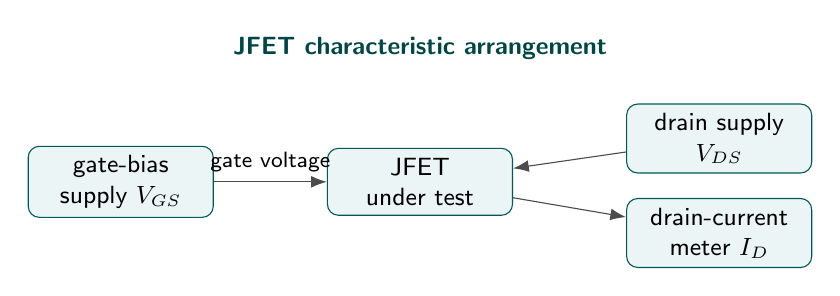
\begin{tikzpicture}[box/.style={draw=teal!70!black,fill=teal!8,rounded corners,minimum width=2.35cm,minimum height=.85cm,align=center,font=\sffamily\small},a/.style={-{Latex[length=2mm]},draw=black!70}]
\node[font=\sffamily\bfseries\small,text=teal!55!black] at (0,1.7) {JFET characteristic arrangement};
\node[box] (gate) at (-3.8,0) {gate-bias\\supply $V_{GS}$};
\node[box] (fet) at (0,0) {JFET\\under test};
\node[box] (drain) at (3.8,.55) {drain supply\\$V_{DS}$};
\node[box] (meter) at (3.8,-.65) {drain-current\\meter $I_D$};
\draw[a] (gate)--node[above,font=\sffamily\footnotesize]{gate voltage} (fet);
\draw[a] (drain)--(fet); \draw[a] (fet)--(meter);
\end{tikzpicture}
\end{document}
